\documentclass[a4paper,12pt]{article}
\usepackage[a4paper, margin=1in]{geometry}
\usepackage{graphicx}
\usepackage{amsmath, amssymb}
\usepackage{booktabs}
\usepackage{caption}
\usepackage{subcaption}
\usepackage{float}
\usepackage{indentfirst}
\usepackage{hyperref}

\title{EC332 - Homework 2}
\author{Zeynep Bozoklu}
\date{\today}

\begin{document}

\maketitle


\begin{figure}[H]
  \centering
  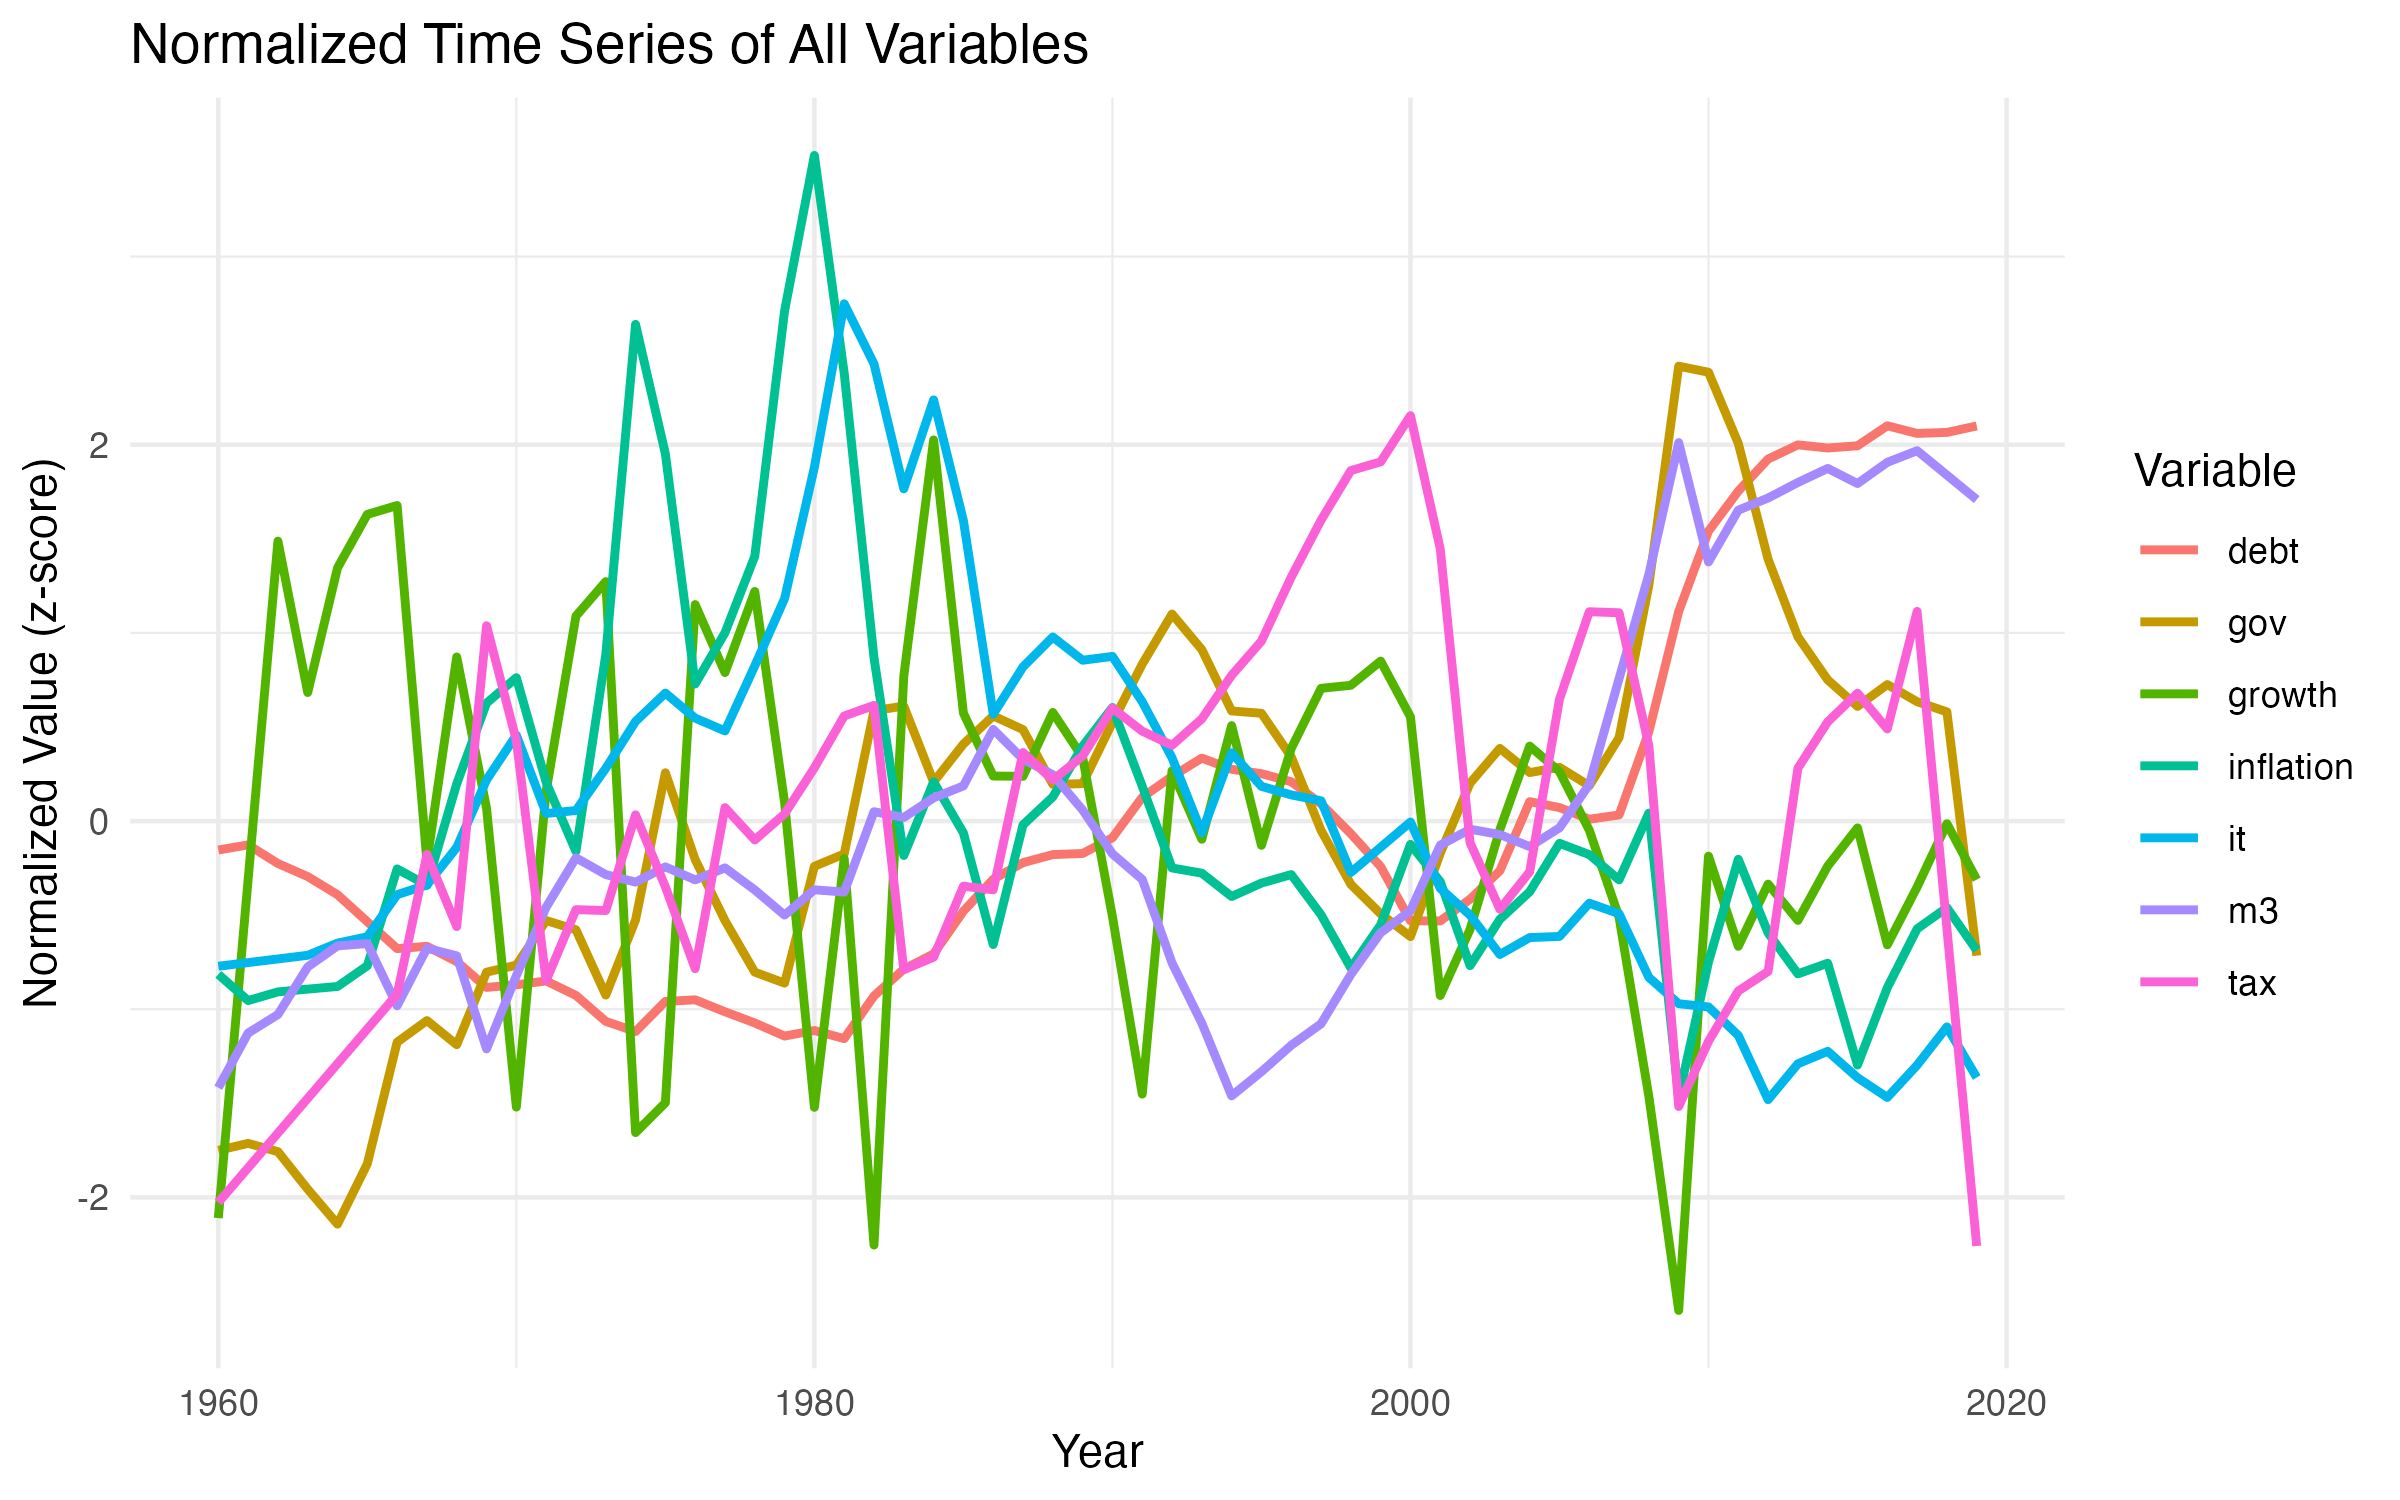
\includegraphics[width=0.9\textwidth]{../results/all_variables_normalized_plot.png}
  \caption{Normalized Initial Plot}
\end{figure}


\section{}
The table below presents the order of integration for all variables, determined by ADF and PP tests.


% Table created by stargazer v.5.2.3 by Marek Hlavac, Social Policy Institute. E-mail: marek.hlavac at gmail.com
% Date and time: Fri, Mar 21, 2025 - 15:47:30
\begin{table}[!htbp] \centering 
  \caption{Stationarity Test Results} 
  \label{} 
\begin{tabular}{@{\extracolsep{5pt}} cccc} 
\\[-1.8ex]\hline 
\hline \\[-1.8ex] 
 & Variable & ADF\_Integration\_Order & PP\_Integration\_Order \\ 
\hline \\[-1.8ex] 
debt & debt & $2$ & $1$ \\ 
gov & gov & $1$ & $1$ \\ 
tax & tax & $1$ & $1$ \\ 
growth & growth & $0$ & $0$ \\ 
inflation & inflation & $1$ & $1$ \\ 
m3 & m3 & $2$ & $1$ \\ 
it & it & $1$ & $1$ \\ 
\hline \\[-1.8ex] 
\end{tabular} 
\end{table} 


The results indicate that \textit{growth} is stationary at level (\(I(0)\)), while \textit{gov}, \textit{tax}, \textit{inflation}, and \textit{it} are stationary after first differencing (\(I(1)\)). However, \textit{debt} and \textit{m3} show conflicting results between the tests, with ADF suggesting second-order integration (\(I(2)\)) and PP suggesting first-order integration (\(I(1)\)). 

To resolve this discrepancy, additional KPSS tests were conducted for \textit{debt} and \textit{m3}. Since the KPSS test assumes stationarity under the null hypothesis, each variable was tested at levels, first differences, and second differences. The results reject stationarity at levels but fail to reject it at the first difference for both variables, indicating that they are stationary after first differencing.


% Table created by stargazer v.5.2.3 by Marek Hlavac, Social Policy Institute. E-mail: marek.hlavac at gmail.com
% Date and time: Sat, Mar 22, 2025 - 12:41:48
\begin{table}[!htbp] \centering 
  \caption{KPSS Test Results for Debt and M3} 
  \label{} 
\begin{tabular}{@{\extracolsep{5pt}} cccccc} 
\\[-1.8ex]\hline 
\hline \\[-1.8ex] 
 & Variable & KPSS\_Level & KPSS\_Diff1 & KPSS\_Diff2 & Final\_KPSS\_Order \\ 
\hline \\[-1.8ex] 
1 & debt & $0.010$ & $0.088$ & $0.100$ & $1$ \\ 
2 & m3 & $0.010$ & $0.100$ & $0.100$ & $1$ \\ 
\hline \\[-1.8ex] 
\end{tabular} 
\end{table} 


Given the robustness of the PP test and the supporting evidence from the KPSS test, \textit{debt} and \textit{m3} are treated as integrated of order one (\(I(1)\)). Consequently, all non-stationary variables in the dataset are considered \(I(1)\), except for \textit{growth}, which is stationary in levels (\(I(0)\)).



\begin{figure}[H]
  \centering
  \begin{subfigure}[b]{0.32\textwidth}
    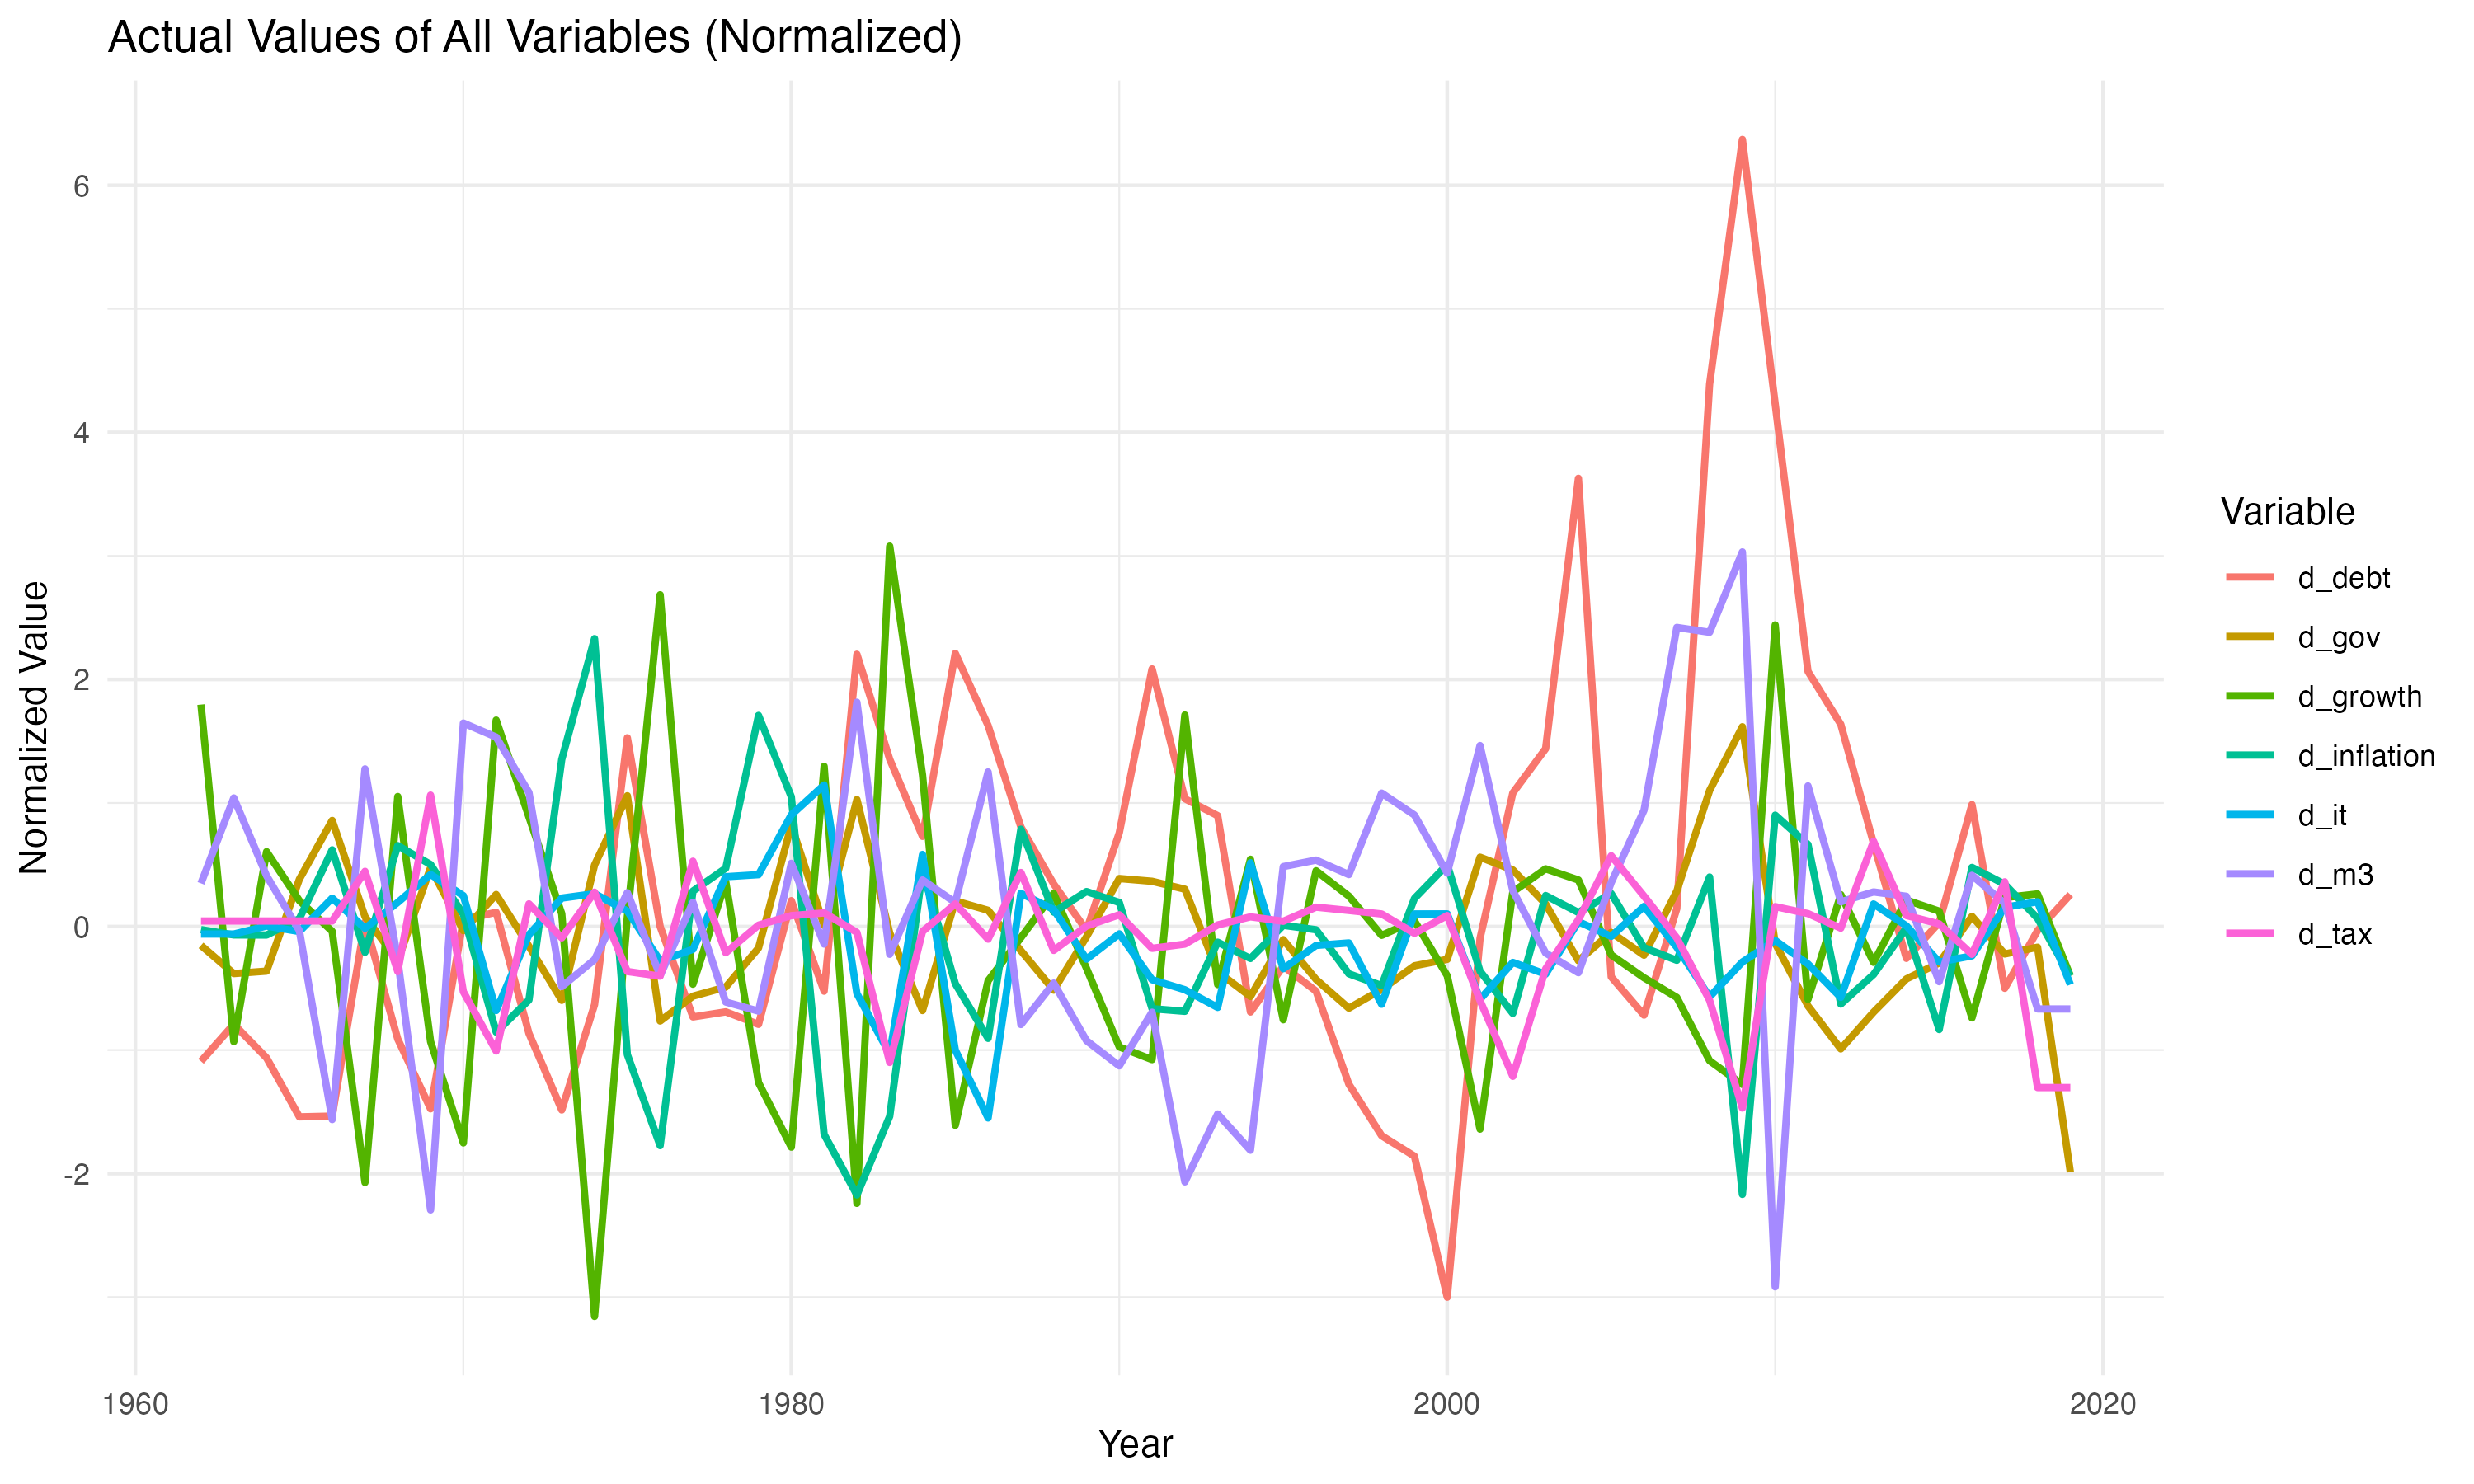
\includegraphics[width=\textwidth]{../results/var1_actual_all.png}
    \caption{Actual (Differenced, Normalized)}
  \end{subfigure}
  \hfill
  \begin{subfigure}[b]{0.32\textwidth}
    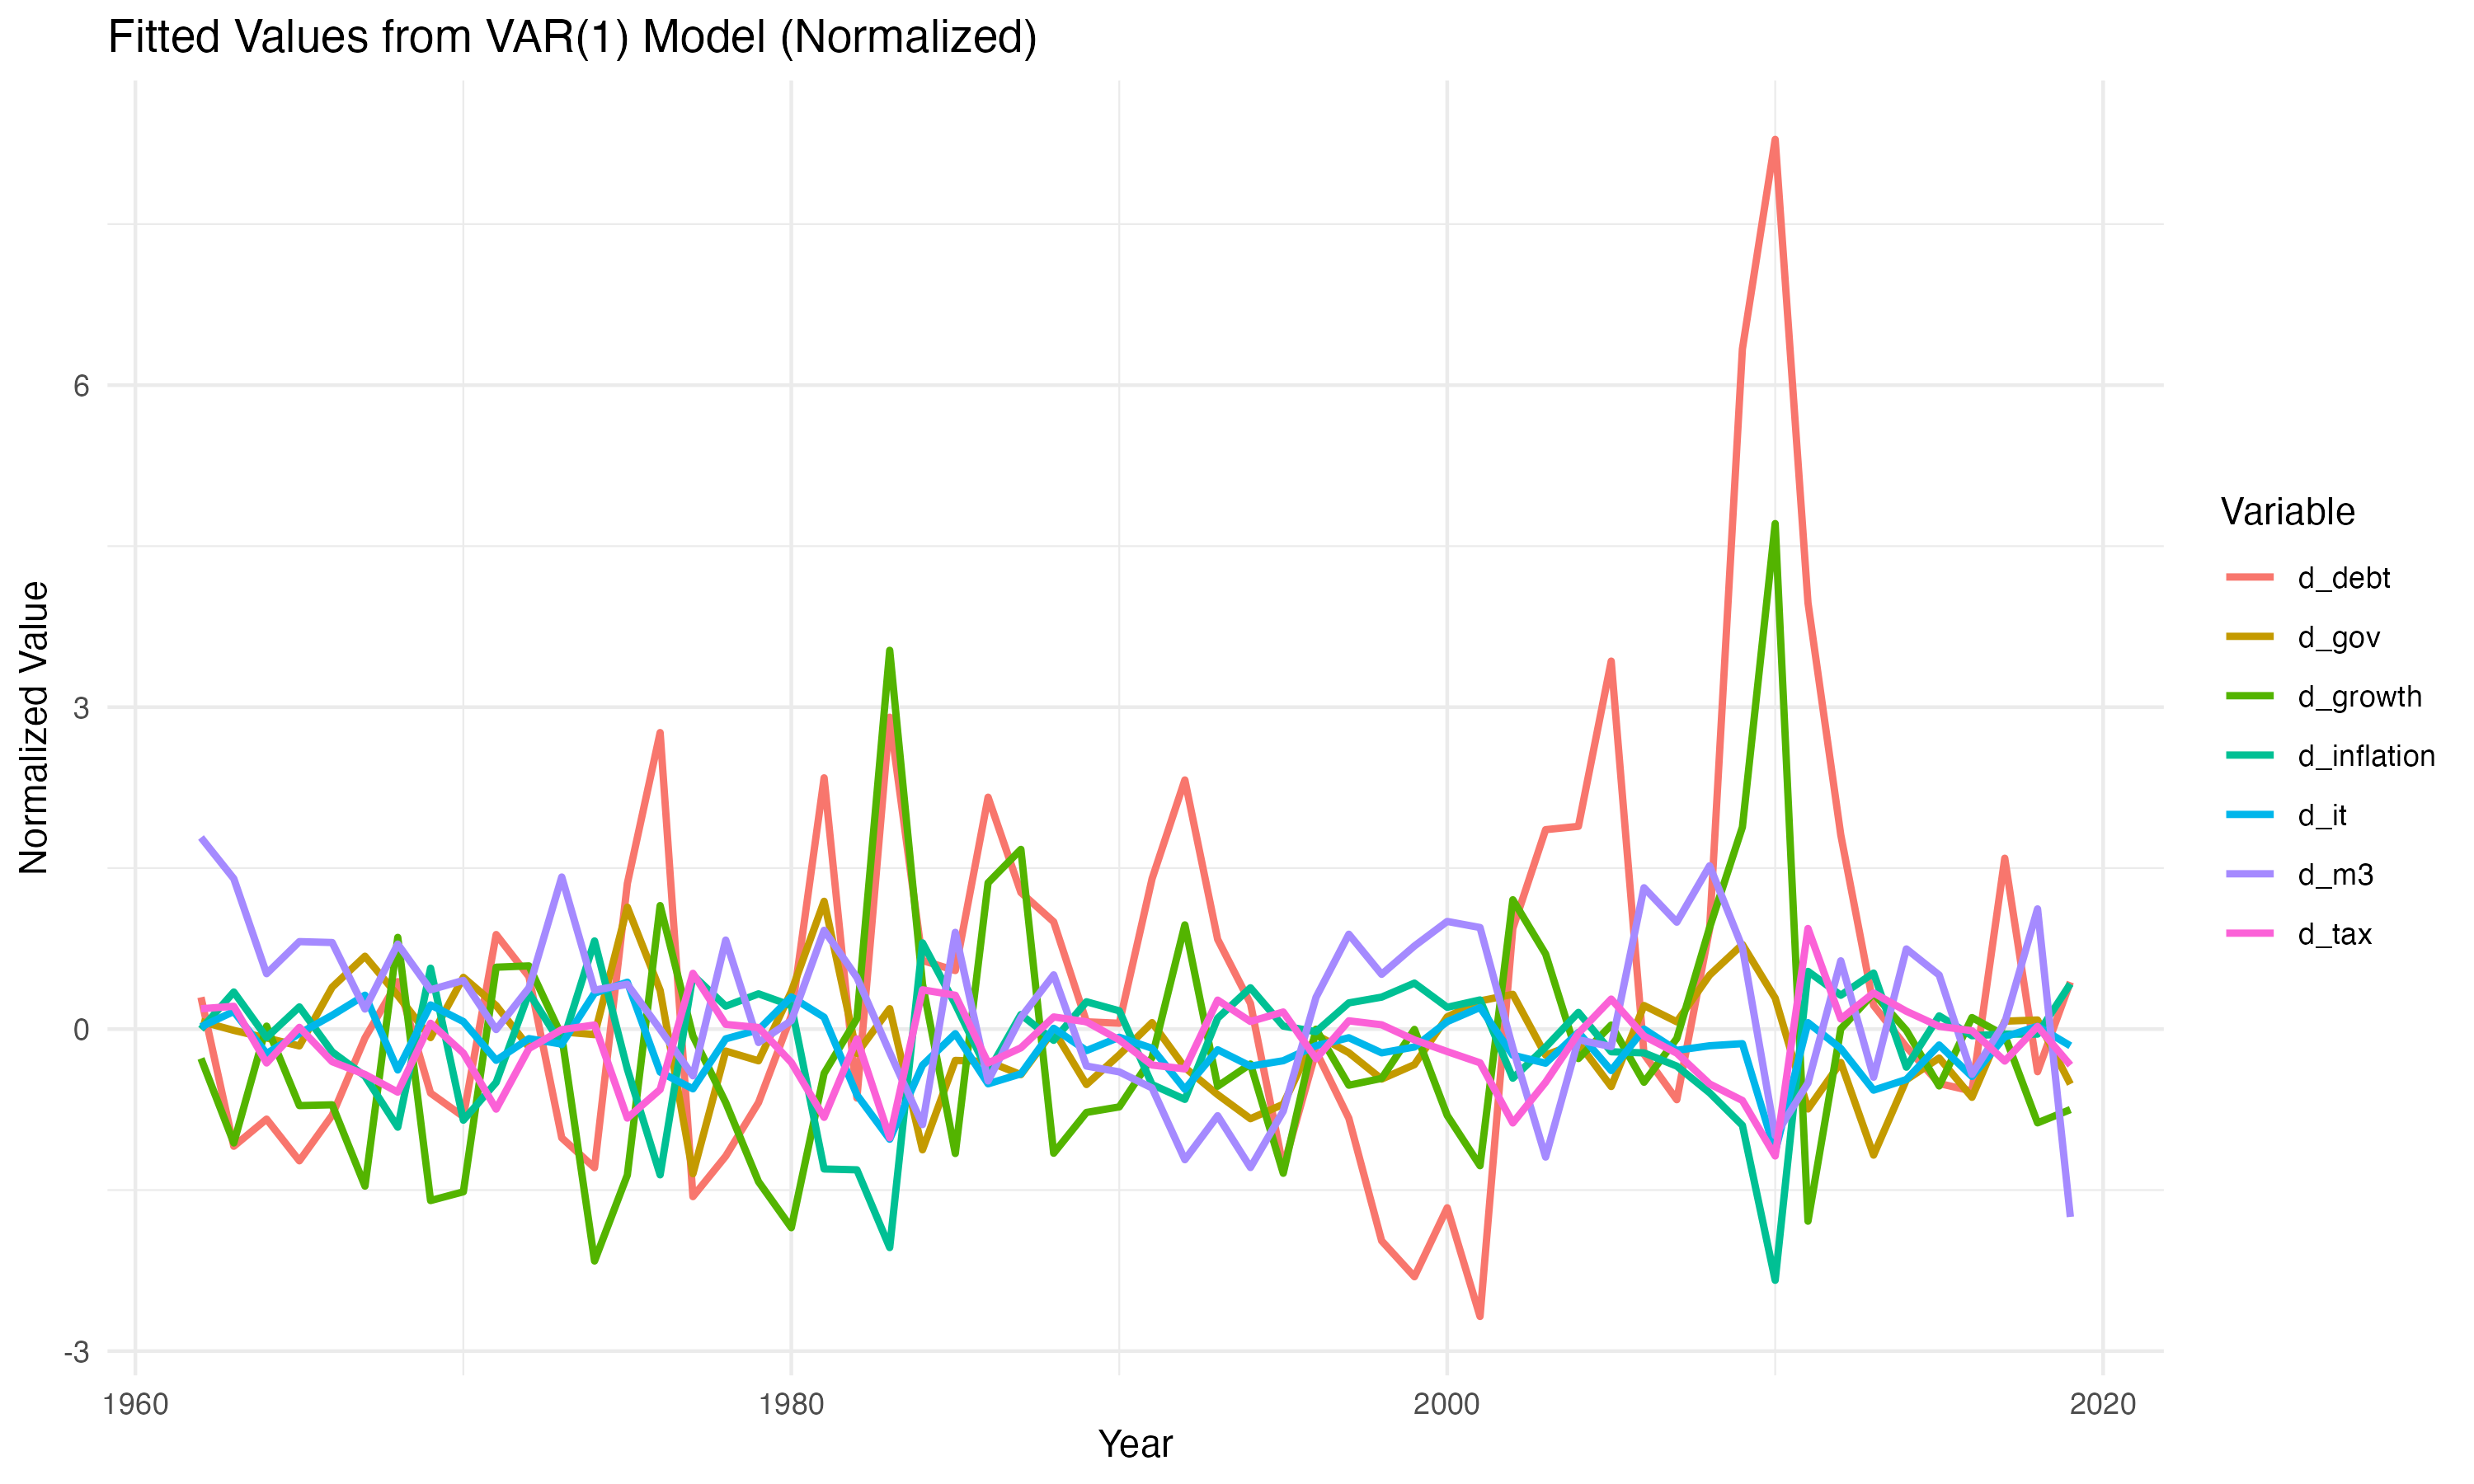
\includegraphics[width=\textwidth]{../results/var1_fitted_all.png}
    \caption{Fitted (VAR(1))}
  \end{subfigure}
  \hfill
  \begin{subfigure}[b]{0.32\textwidth}
    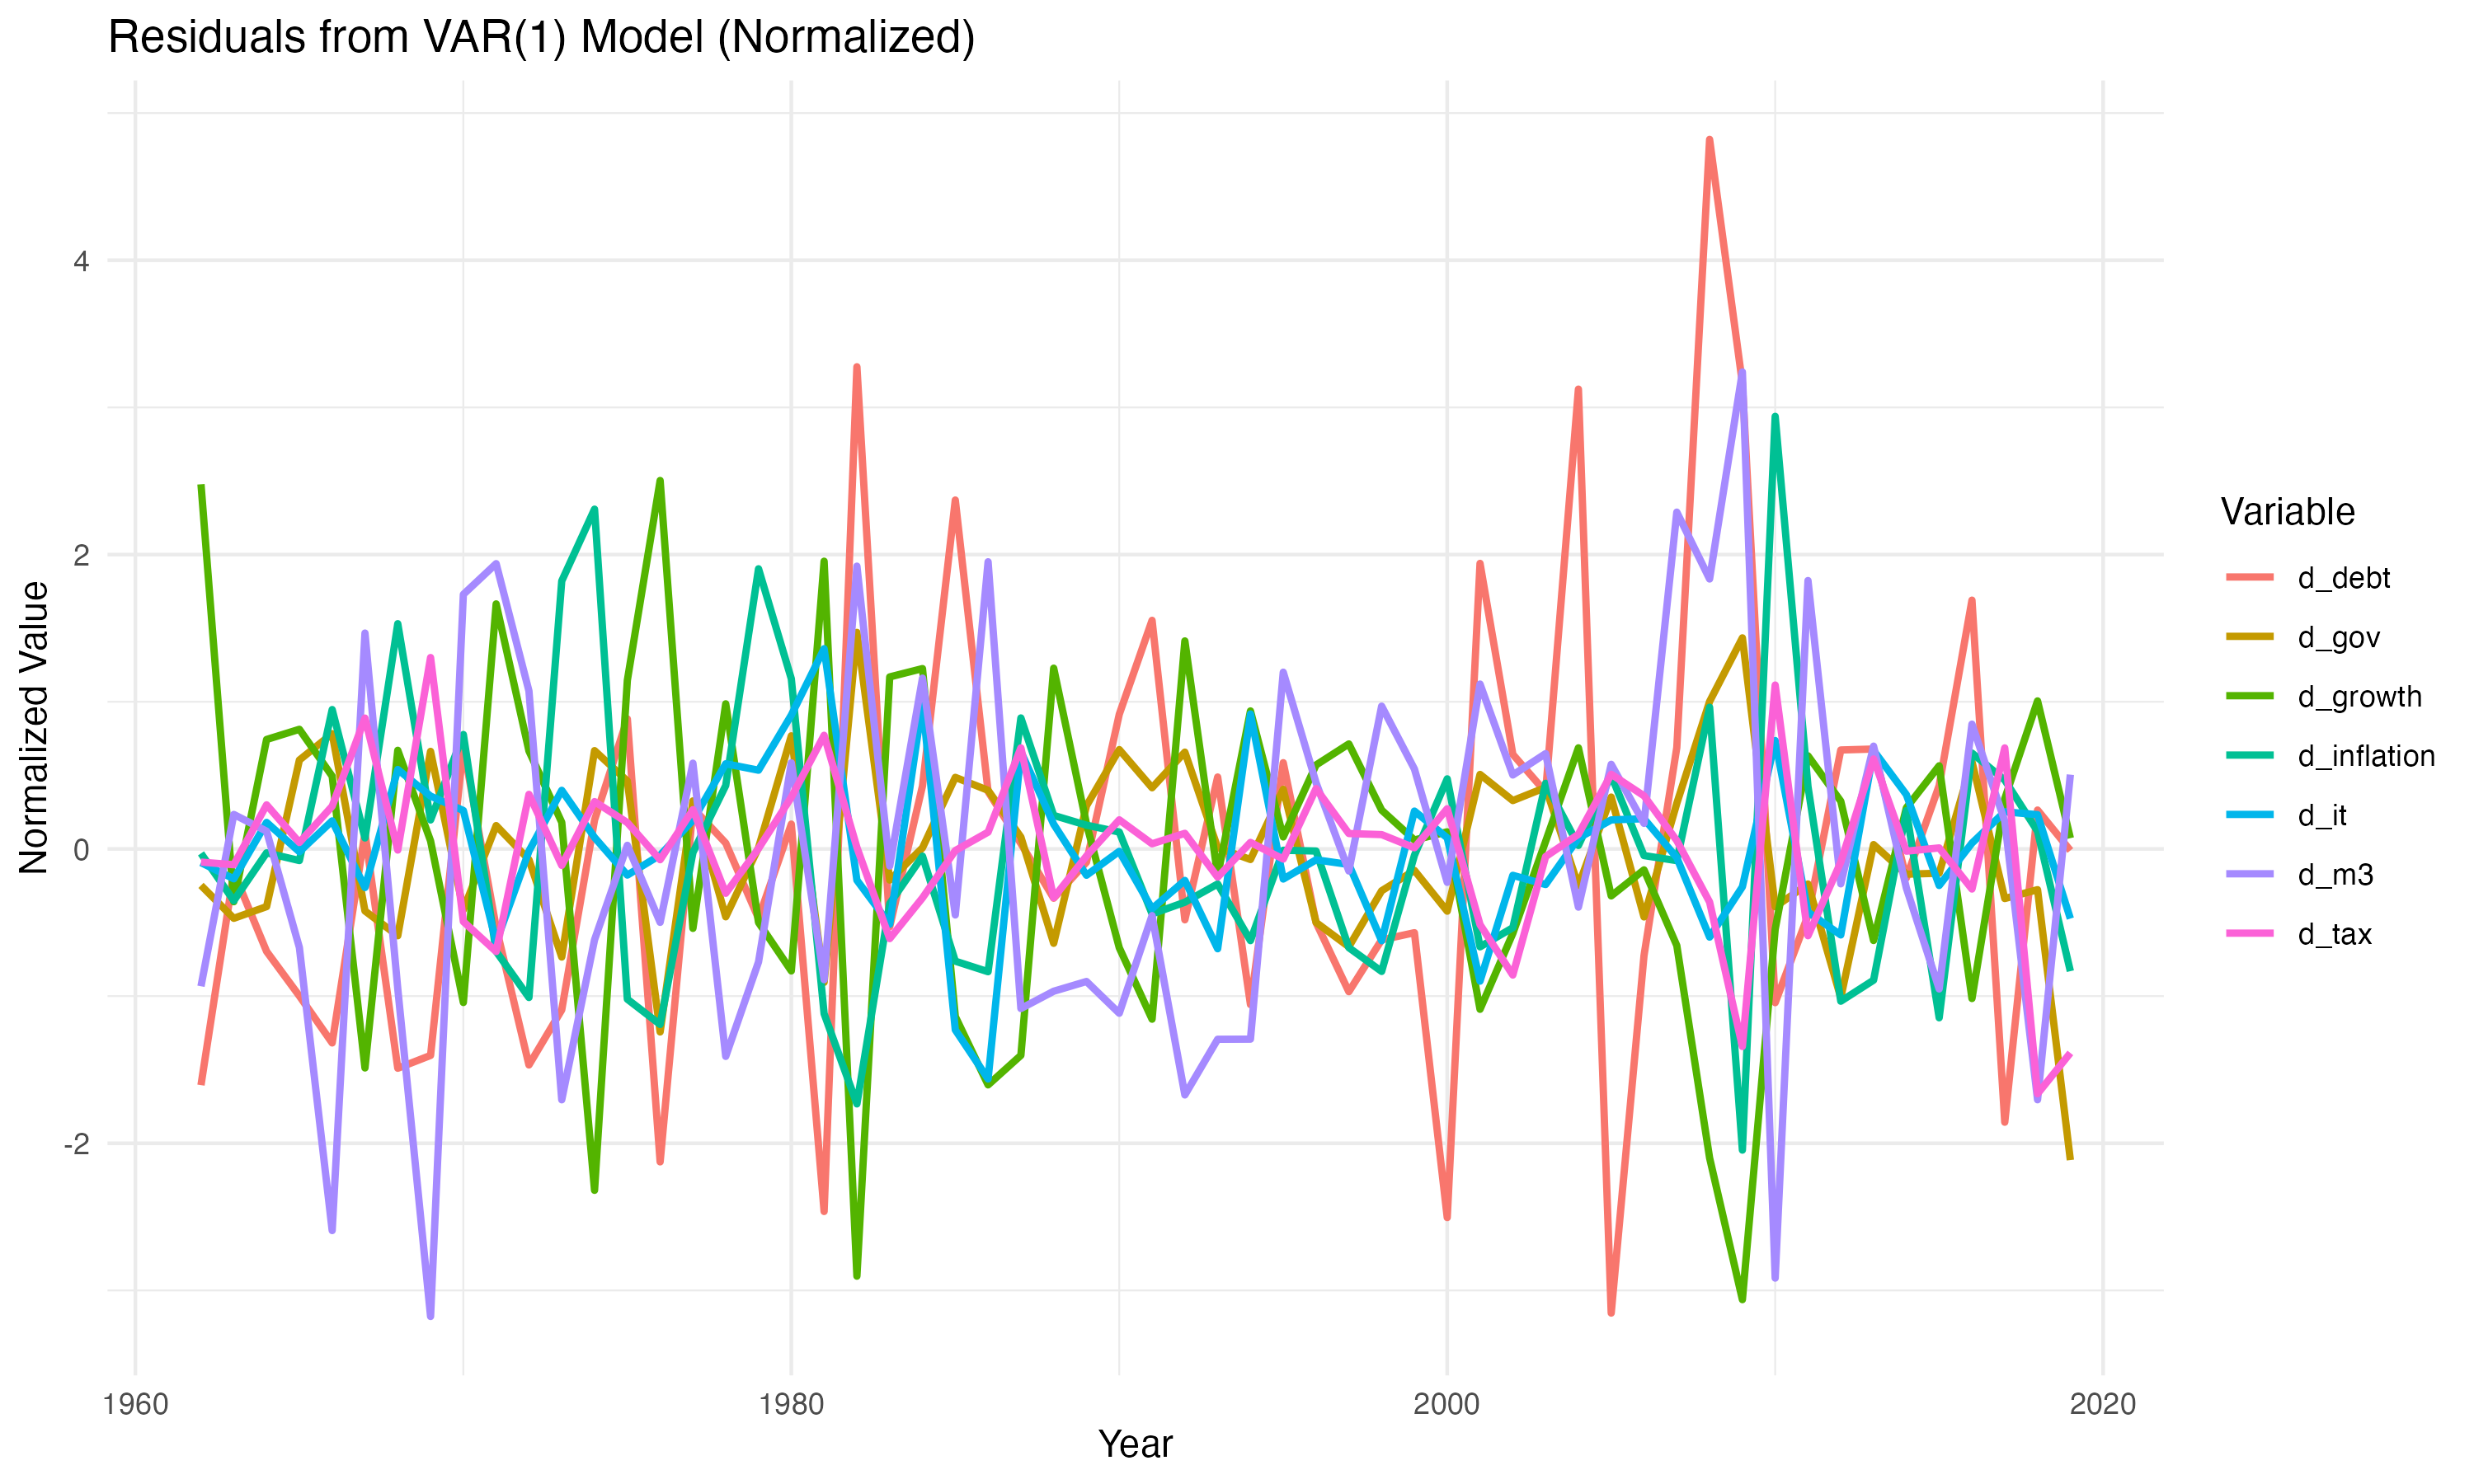
\includegraphics[width=\textwidth]{../results/var1_residuals_all.png}
    \caption{Residuals}
  \end{subfigure}
  \caption{Actual, Fitted, and Residual Series from VAR(1) Model (Normalized)}
  \label{fig:var1_allseries}
\end{figure}

\section{}


Lag length selection was performed using AIC, HQ, SC, and FPE criteria. These are commonly used information criteria that guide model specification by balancing model fit and complexity. For each criterion, the lag length with the \textit{lowest} value is considered optimal. 

The Akaike Information Criterion (AIC) and Final Prediction Error (FPE) prioritize model fit, which may lead to selecting more lags. In contrast, the Schwarz Criterion (SC or BIC) and Hannan-Quinn Criterion (HQ) impose heavier penalties for additional lags and often favor more parsimonious models. 

In this case, all criteria consistently suggested using a single lag across the range of lag lengths considered. Therefore, a VAR(1) specification is chosen for estimation in the following analysis.


% Table created by stargazer v.5.2.3 by Marek Hlavac, Social Policy Institute. E-mail: marek.hlavac at gmail.com
% Date and time: Sat, Mar 22, 2025 - 18:24:40
\begin{table}[!htbp] \centering 
  \caption{VAR Lag Length Selection Criteria} 
  \label{} 
\begin{tabular}{@{\extracolsep{5pt}} cccccc} 
\\[-1.8ex]\hline 
\hline \\[-1.8ex] 
 & Lag & AIC(n) & HQ(n) & SC(n) & FPE(n) \\ 
\hline \\[-1.8ex] 
1 & $1$ & $4.258$ & $5.054$ & $6.321$ & $71.786$ \\ 
2 & $2$ & $4.716$ & $6.208$ & $8.584$ & $124.131$ \\ 
3 & $3$ & $5.116$ & $7.304$ & $10.788$ & $236.811$ \\ 
4 & $4$ & $5.557$ & $8.441$ & $13.034$ & $625.460$ \\ 
5 & $5$ & $4.829$ & $8.408$ & $14.111$ & $863.874$ \\ 
\hline \\[-1.8ex] 
\end{tabular} 
\end{table} 


\section{}

Granger causality tests are used to identify predictive relationships among variables: specifically, whether past values of one variable help forecast another. A p-value below 0.05 indicates that the null hypothesis of "no Granger causality" can be rejected, meaning that one variable Granger-causes another.

The heatmap below visualizes the p-values from pairwise Granger causality tests among all stationary variables. Significant relationships (p $<$ 0.05) are marked with an asterisk.

\begin{figure}[H]
  \centering
  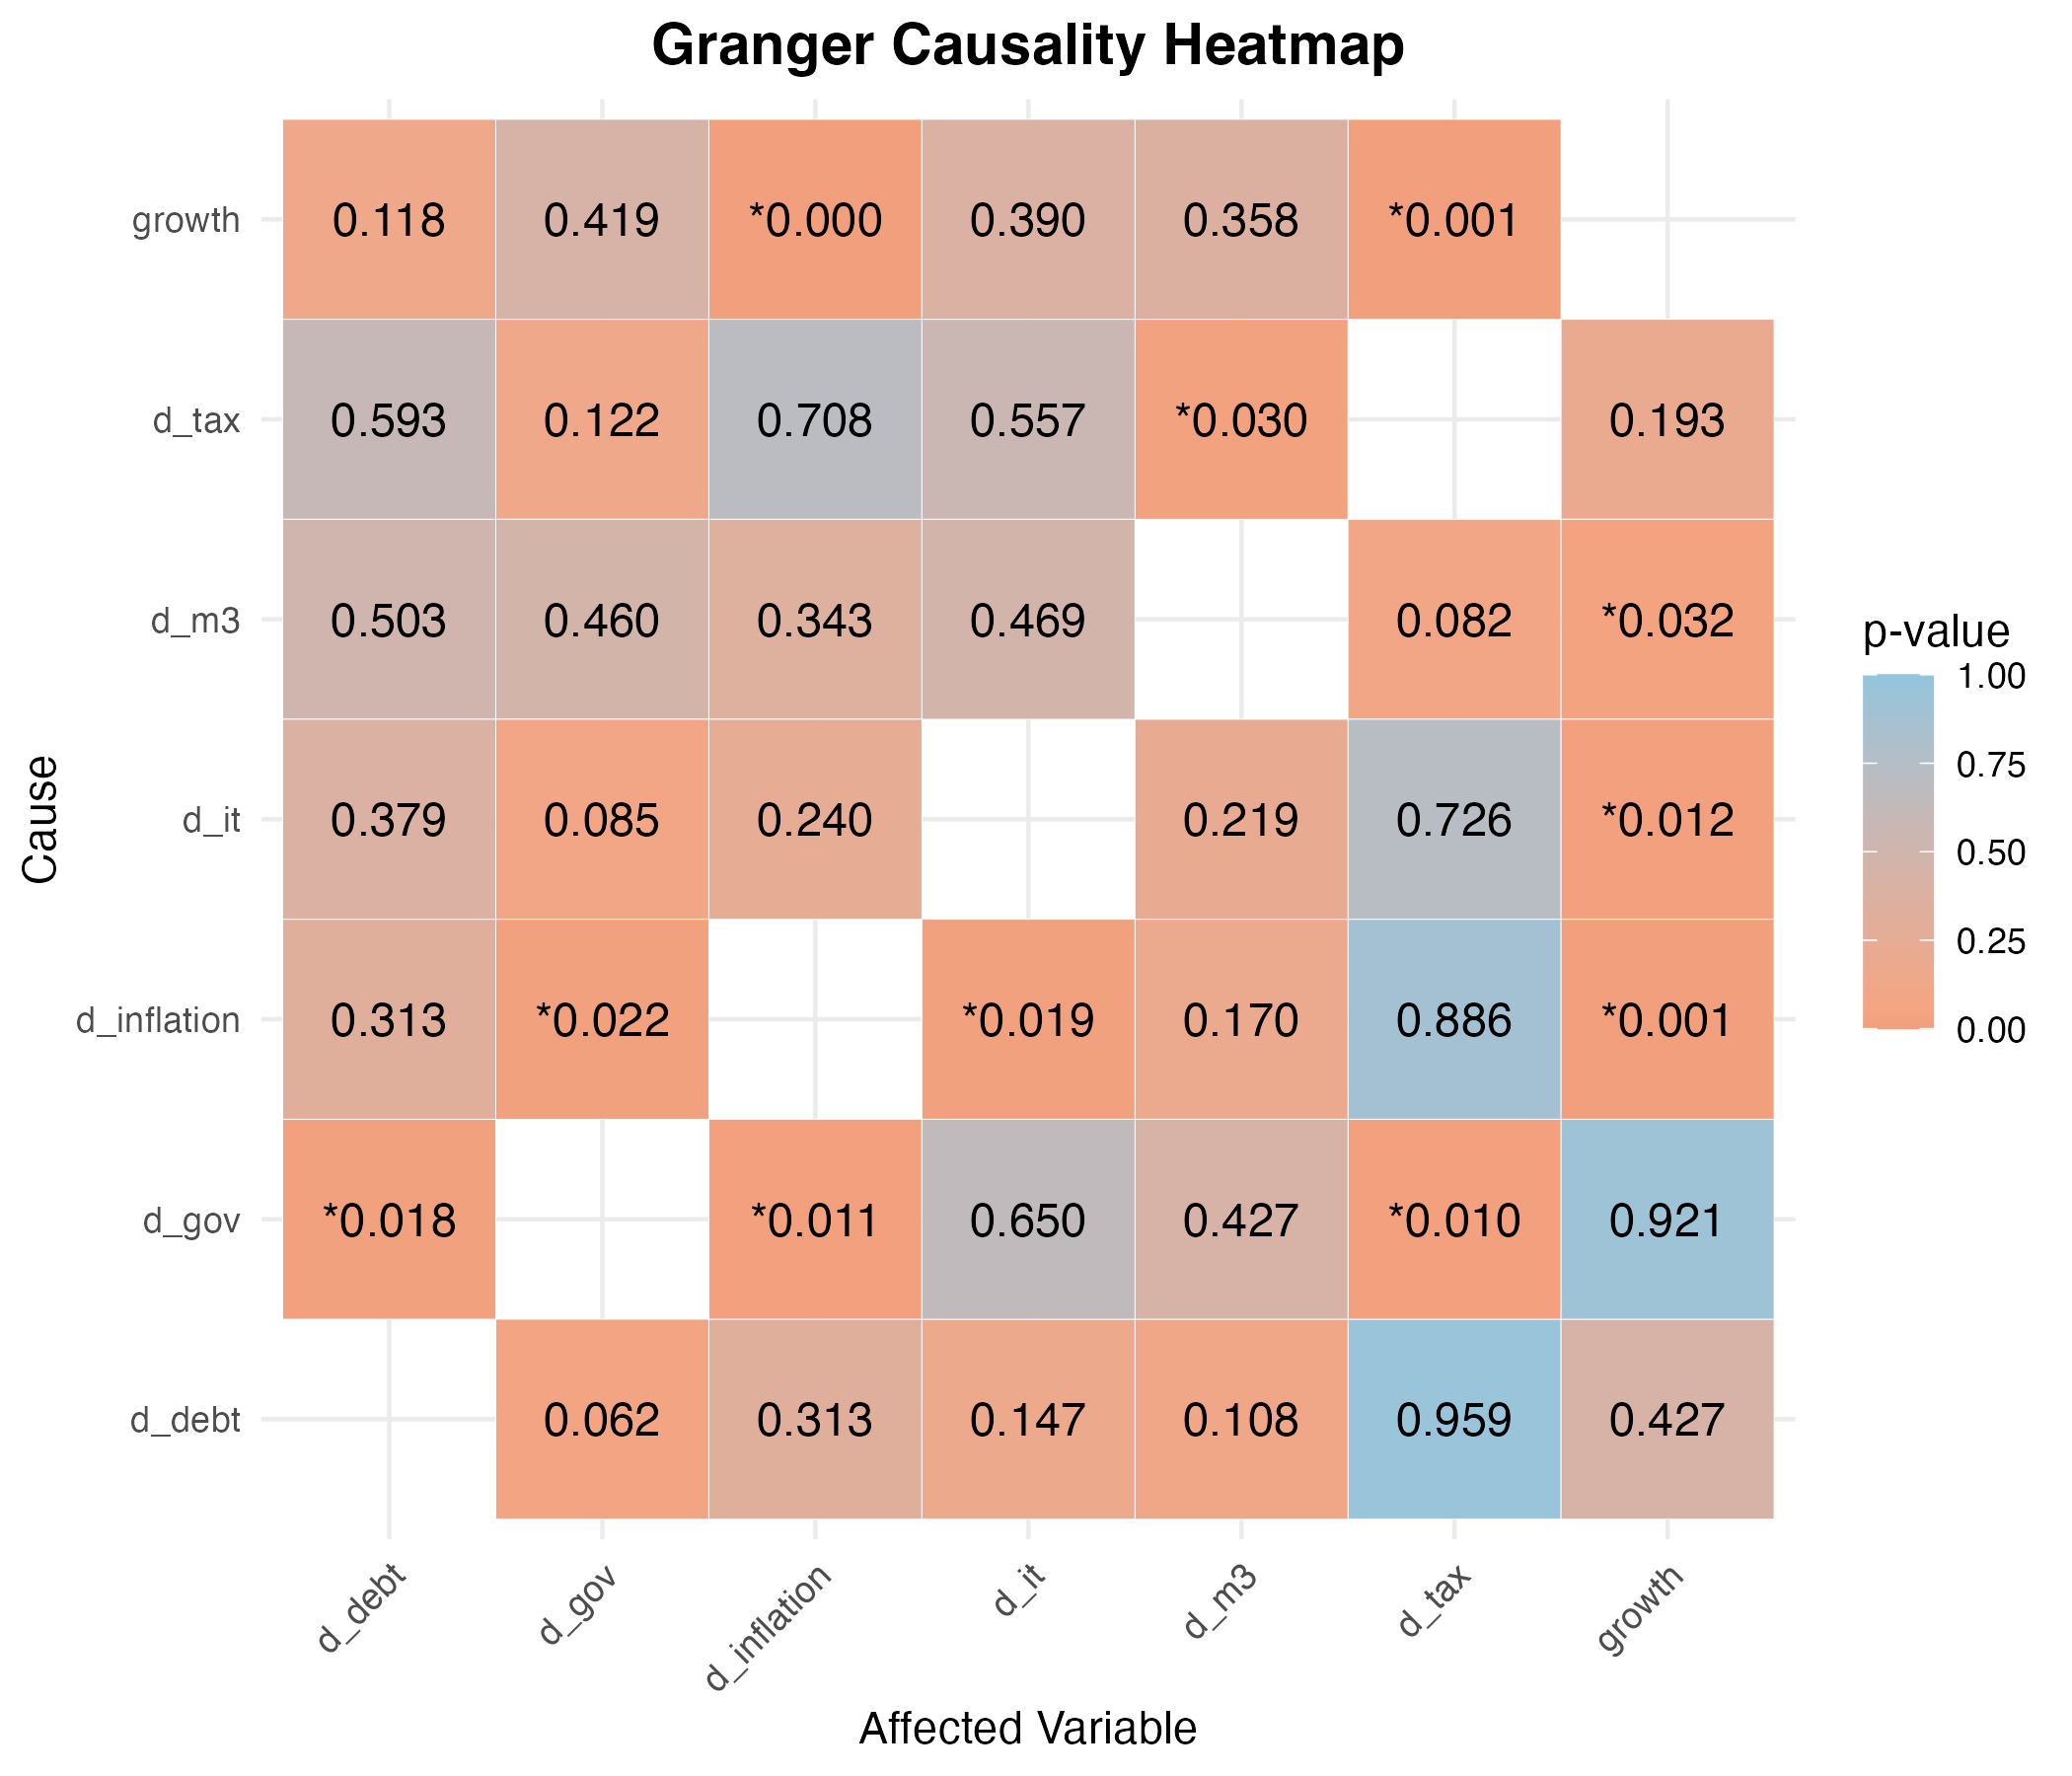
\includegraphics[width=0.44\textwidth]{../results/granger_causality_heatmap.png}
  \caption{Granger Causality Test Results (p-values)}
\end{figure}

\textbf{Summary of Significant Granger-Causal Relationships}

\begin{itemize}
  \item \textbf{growth} $\rightarrow$ d\_inflation, d\_tax
  \item \textbf{d\_tax} $\rightarrow$ d\_m3
  \item \textbf{d\_m3} $\rightarrow$ growth
  \item \textbf{d\_it} $\rightarrow$ growth
  \item \textbf{d\_inflation} $\rightarrow$ d\_gov, d\_it, growth
  \item \textbf{d\_gov} $\rightarrow$ d\_debt, d\_inflation, d\_tax
  \item \textbf{d\_debt} $\rightarrow$ None (no significant Granger causality)
\end{itemize}

\textbf{Interpretation and Economic Intuition}

\begin{itemize}
  \item \textbf{Growth Granger-causing inflation and tax revenue} reflects demand-side dynamics. Strong growth often leads to increased demand, pushing up prices (demand-pull inflation), and boosts tax revenues through higher income and consumption.
  
  \item \textbf{Tax revenue Granger-causing money supply} may suggest policy coordination. Rising taxes might reduce deficits, influencing liquidity needs or central bank responses.

  \item \textbf{Money supply Granger-causing growth} aligns with classical monetary theory. Greater liquidity supports investment and consumption, which drives output.

  \item \textbf{Interest rate Granger-causing growth} captures the standard monetary transmission mechanism. Changes in interest rates influence borrowing and investment behavior, affecting aggregate demand.

  \item \textbf{Inflation Granger-causing spending, interest rates, and growth} suggests inflation acts as a policy signal. Governments and central banks may react to inflation by adjusting fiscal and monetary policy. Additionally, inflation could influence output via cost-push effects.

  \item \textbf{Government spending Granger-causing debt, inflation, and tax revenue} reflects standard macroeconomic channels. Fiscal expansions increase debt when deficit-financed, stimulate demand and inflation, and boost tax revenue via multiplier effects.

  \item \textbf{Debt not Granger-causing any other variable} suggests that debt acts as a lagging indicator—reacting to changes in growth or spending rather than driving them in the short run.
\end{itemize}

These results collectively validate classical macroeconomic transmission mechanisms and show how fiscal and monetary variables interact with real economic outcomes.

\section{}

Impulse response functions (IRFs) trace the effect of a one-time shock to one variable on the current and future values of all variables in a VAR system. Using the VAR(1) model estimated earlier, the dynamic responses of all variables to one-standard-deviation shocks in each variable were analyzed.

\begin{figure}[H]
  \centering
  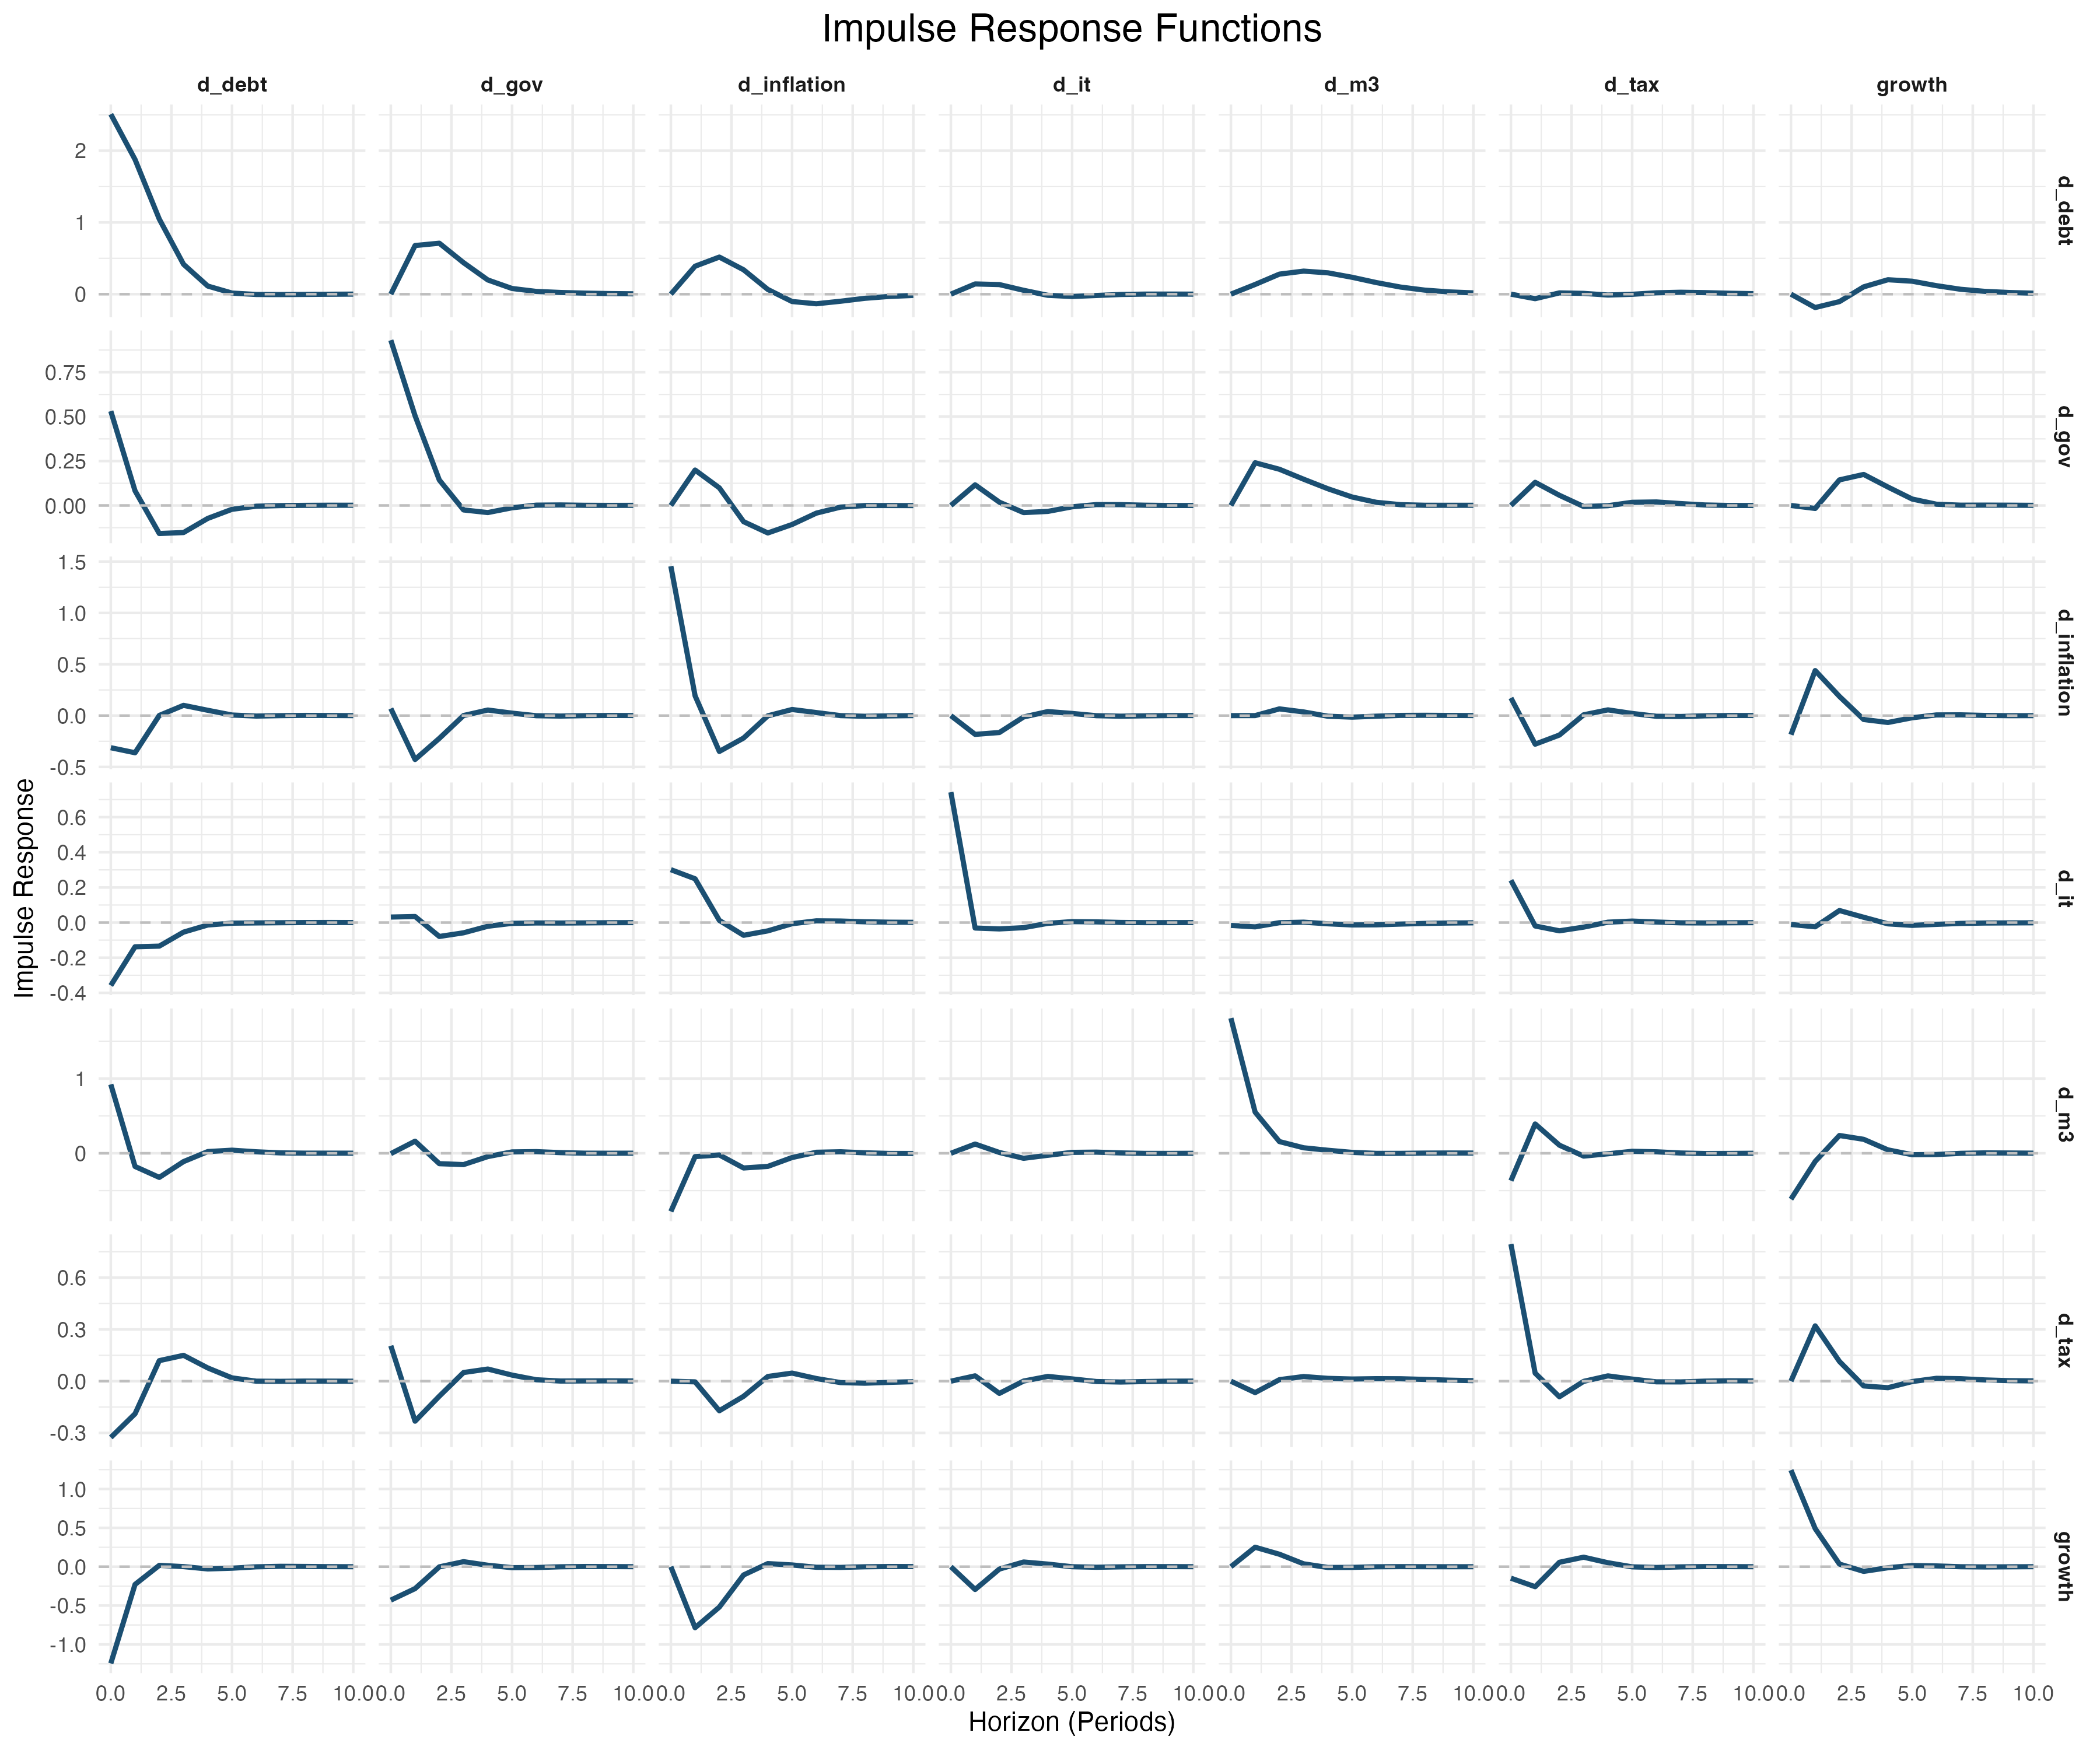
\includegraphics[width=0.9\textwidth]{../results/irf_faceted_plot.png}
  \caption{Impulse Response Functions (10 Periods Ahead)}
\end{figure}

Each row in the IRF plot represents a one-time shock to a given variable, and each column shows how the remaining variables respond over ten periods.

\begin{itemize}
  \item \textbf{Government Spending Shocks (d\_gov):}
  Boost public debt and mildly raise output and inflation. 
  This aligns with a standard fiscal multiplier, but comes at the cost of higher debt.

  \item \textbf{Tax Shocks (d\_tax):}
  Lower debt (via increased revenue) without reducing output.
  Inflation and interest rates remain near baseline, indicating limited macro disruption.

  \item \textbf{Debt Shocks (d\_debt):}
  Have mild real-side effects. A debt increase does not strongly affect inflation, interest rates, or growth,
  suggesting debt is more reactive than causal in this system.

  \item \textbf{Interest Rate Shocks (d\_it):}
  Cause no contraction in output and do not strongly reduce inflation,
  implying a relatively weak monetary transmission channel. Public debt declines slightly as borrowing becomes costlier.

  \item \textbf{Money Supply Shocks (d\_m3):}
  Show initial contractionary impact on inflation or output, suggesting either sterilization or weak short-run monetary transmission.
  Interest rates remain largely unchanged, and fiscal variables are not strongly affected.

  \item \textbf{Inflation Shocks (d\_inflation):}
  Do not trigger a forceful policy response. Government spending dips, but interest rates barely move,
  and output may even see a brief positive bump.

  \item \textbf{Growth Shocks (growth):}
A positive output shock reduces both public debt and inflation, suggesting improved fiscal balances and muted price pressures when the economy expands. Other variables, such as government spending, interest rates, and tax revenue, remain near baseline, indicating limited spillovers from growth shocks.

\end{itemize}

\section{}

Forecast Error Variance Decompositions (FEVD) quantify how much of each variable's forecast error variance is explained by its own shocks versus shocks to other variables. Figure~\ref{fig:fevd_area} presents a stacked area plot showing how these contributions evolve from horizon 1 to 10 for key variables.

\begin{figure}[H]
  \centering
  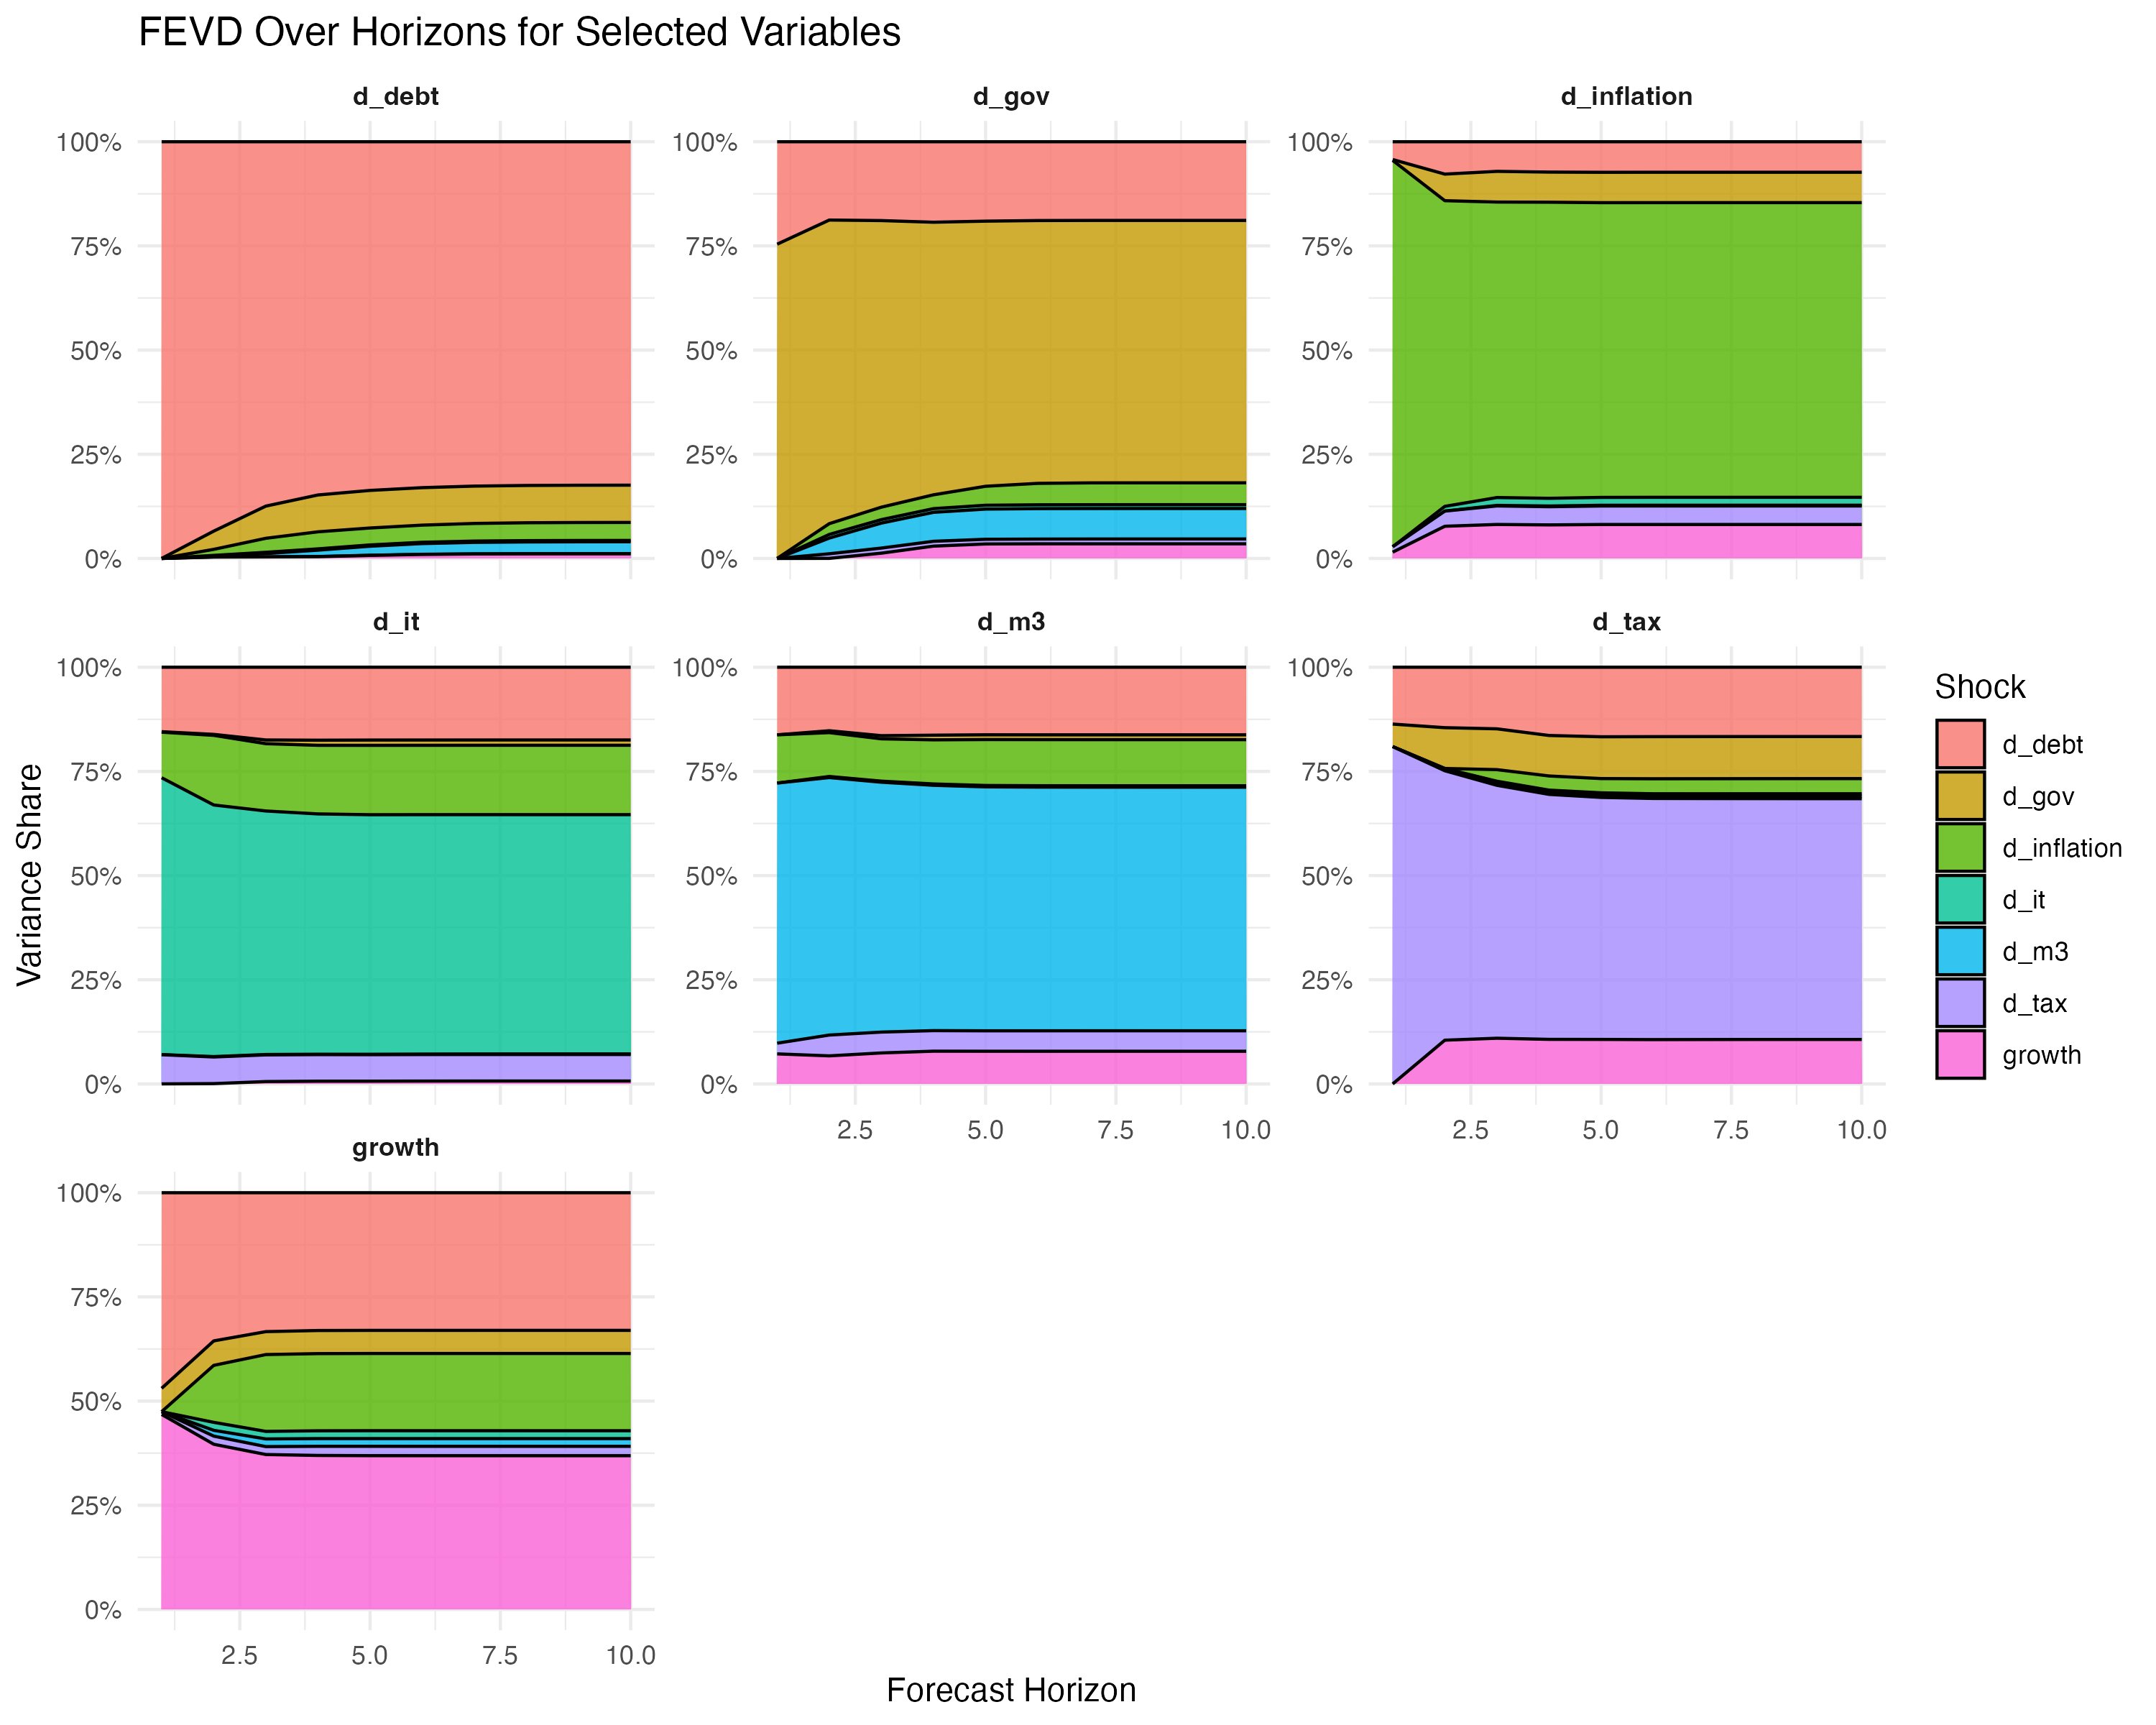
\includegraphics[width=0.8\textwidth]{../results/fevd_stacked_area.png}
  \caption{Forecast Error Variance Decomposition (Stacked Area)}
  \label{fig:fevd_area}
\end{figure}

\begin{itemize}
    \item \textit{\(d\_debt\):} The variance in government debt is primarily driven by shocks to government spending (\(d\_gov\)). This indicates that fiscal policy changes—through their financing and borrowing implications—are the main determinants of debt dynamics.
    
    \item \textit{\(d\_gov\):} Government spending variability is largely explained by debt shocks (\(d\_debt\)). This reciprocal relationship suggests that increases in debt significantly influence fiscal expansion decisions.
    
    \item \textit{\(d\_it\):} The forecast error variance of interest rates is mainly attributable to shocks in debt and inflation (\(d\_debt\) and \(d\_inflation\)), underscoring that monetary policy responses are closely linked to fiscal imbalances and price pressures.
    
    \item \textit{\(d\_m3\):} Money supply fluctuations are largely driven by debt and inflation shocks, implying that changes in the monetary base tend to reflect underlying fiscal imbalances and inflationary pressures.
    
    \item \textit{\(d\_tax\):} Tax revenue variability is significantly influenced by shocks to debt, government spending, and growth. This pattern suggests that fiscal policy and overall economic performance play a key role in determining tax collection.
    
    \item \textit{growth:} Output variability is mainly explained by shocks to debt and inflation, highlighting the importance of fiscal imbalances and price dynamics in shaping real economic activity.
\end{itemize}

\section{}

Forecasts for tax revenue (\textit{d\_tax}) for the years 2020 and 2021 are generated using a univariate AR(1) model estimated in levels. The forecast indicates a slight increase in tax revenue over the two-year horizon, with substantial uncertainty around the estimates.


\begin{table}[!h]
\centering
\begin{tabular}{rrrr}
\toprule
Year & Forecast & 95\% CI Lower & 95\% CI Upper\\
\midrule
2020 & 21.54 & 19.62 & 23.45\\
2021 & 21.48 & 17.63 & 25.33\\
\bottomrule
\end{tabular}
\end{table}




The relatively flat forecast path implies tax revenues are expected to stabilize near their recent levels. However, the wide confidence intervals suggest the forecast is subject to considerable uncertainty. This reflects the limitations of using a simple time series model for forecasting during periods of potential structural change or heightened volatility.

The figure below displays both the historical series and the forecasts, with the 95\% confidence intervals shaded in blue.

\begin{figure}[H]
  \centering
  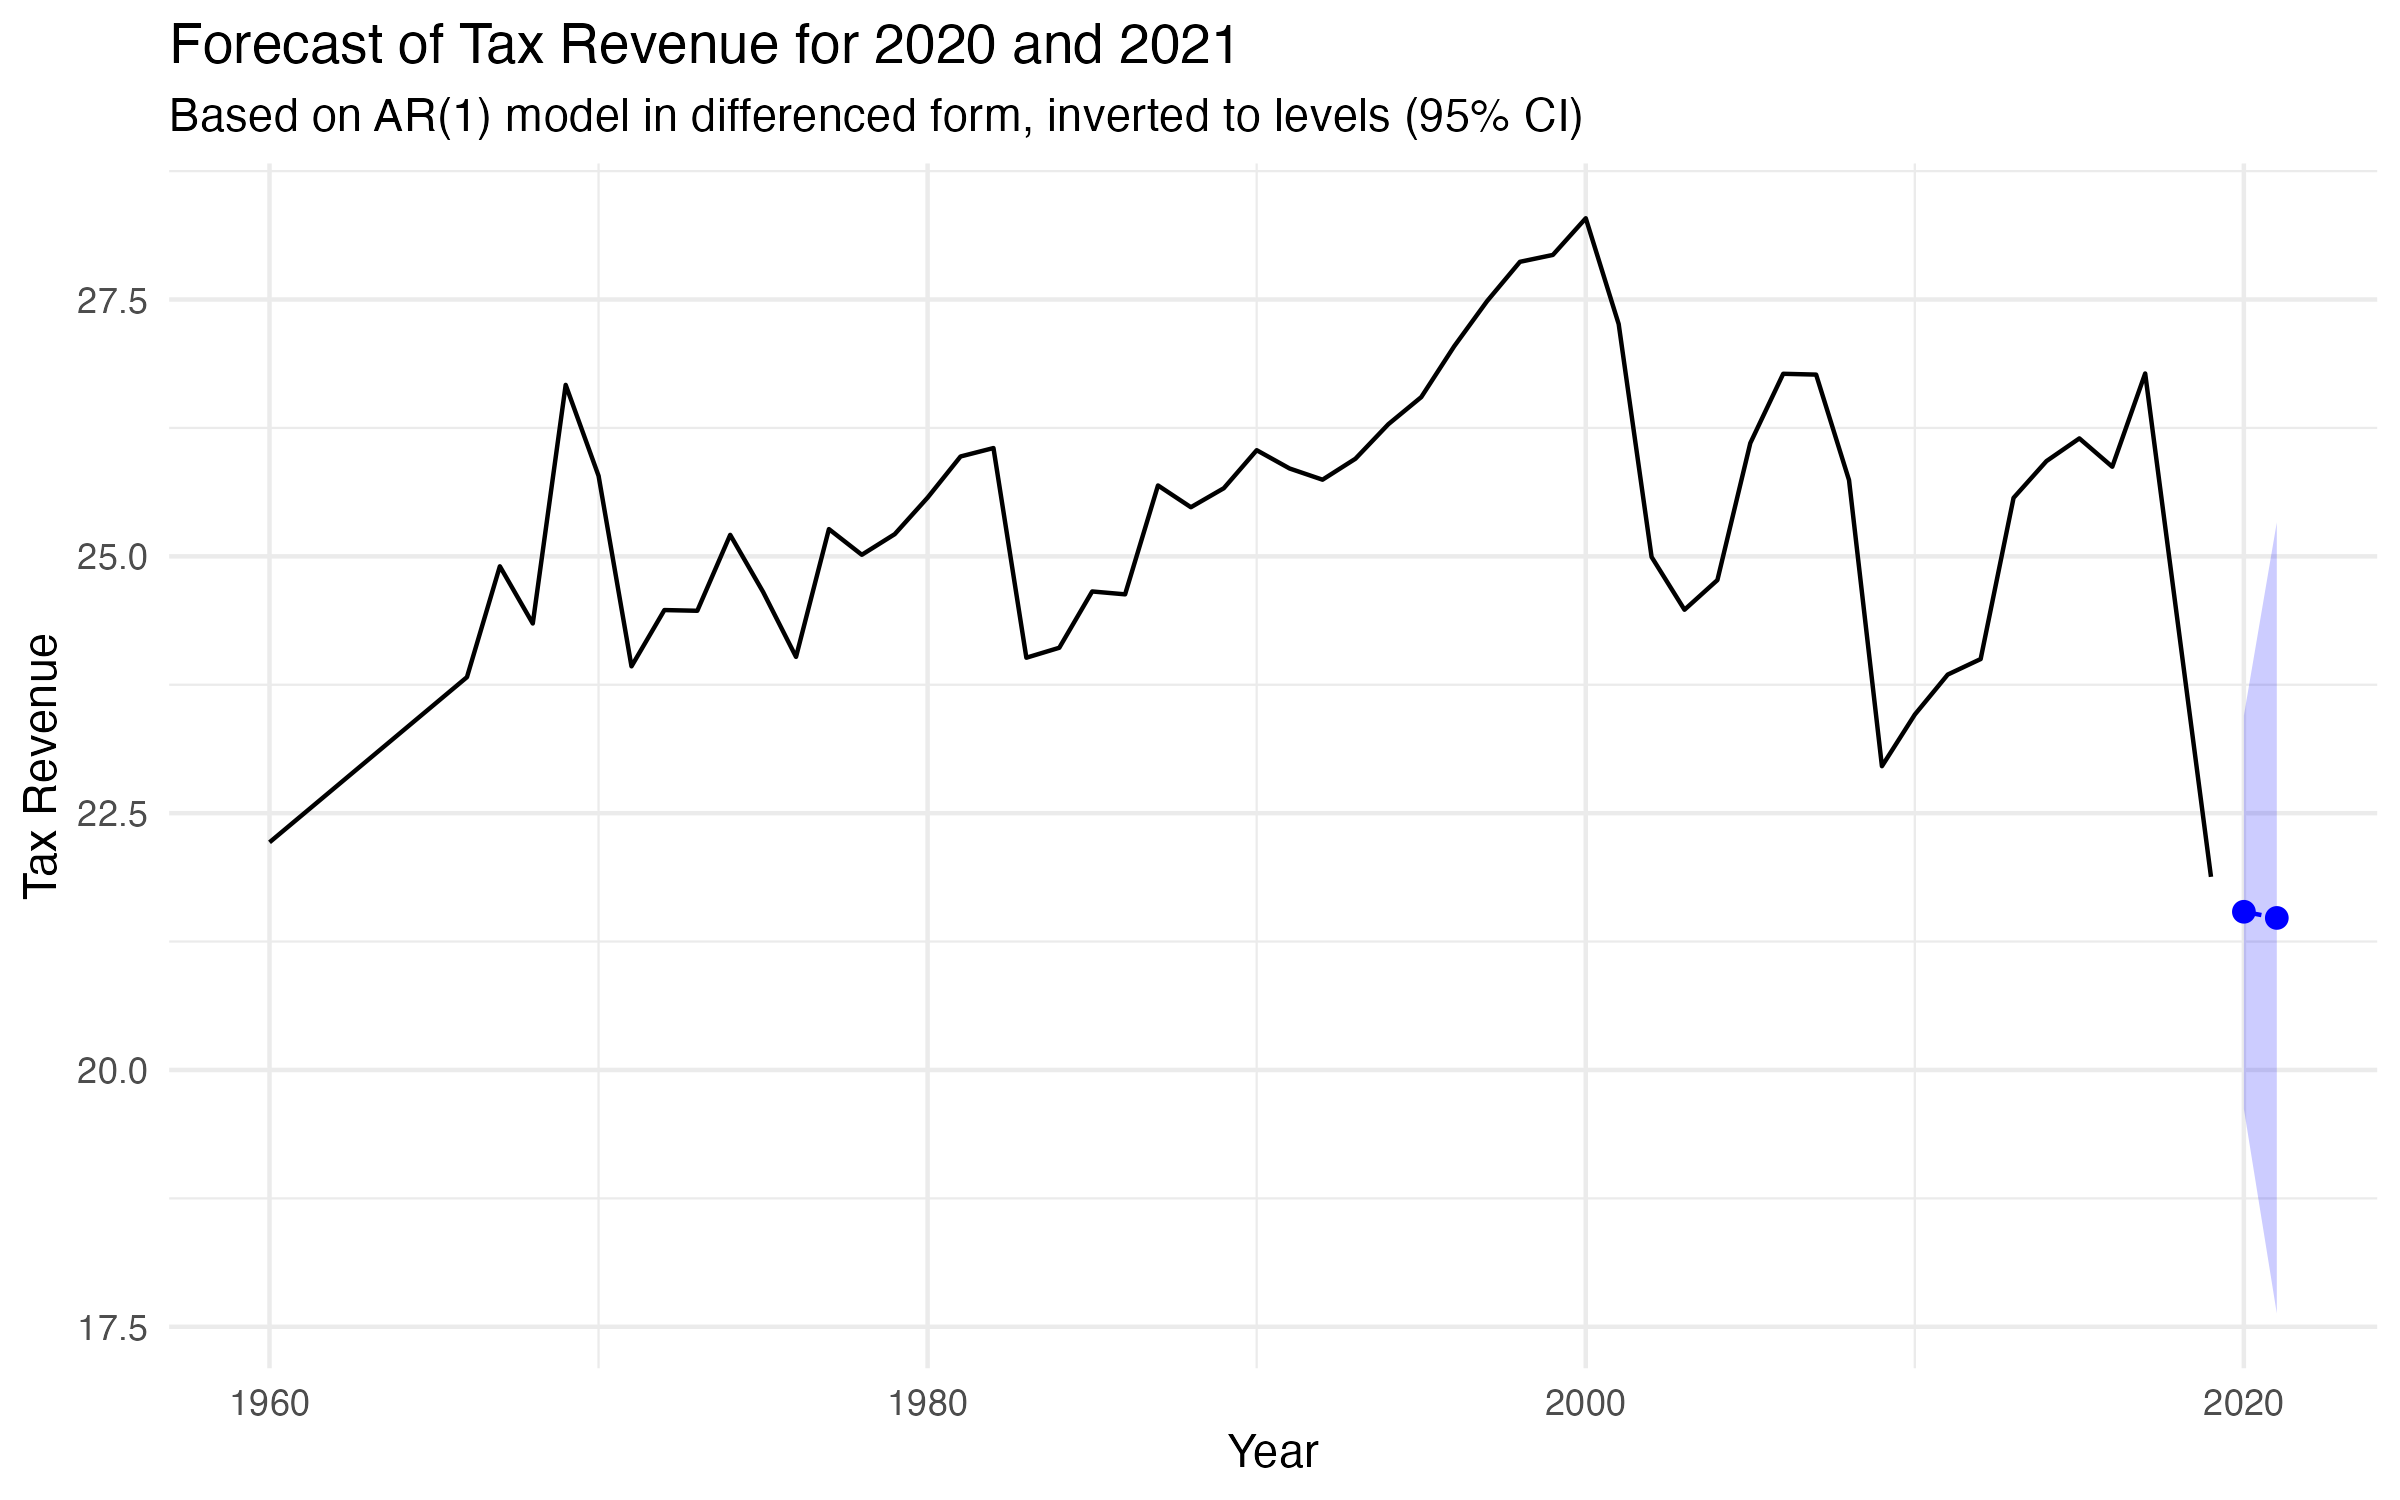
\includegraphics[width=0.85\textwidth]{../results/d_tax_forecast_plot.png}
  \caption{Forecast of Tax Revenue for 2020 and 2021 (Levels)}
\end{figure}













\end{document}
